\chapter{Analysis}

\section{Existing System}

Early days Libraries are managed manually. It required lot of time to record or to retrieve
the details. The employees who have to record the details must perform their job very
carefully. Even a small mistake would create a lot of problems. Security of information is
very less. Report generations of all the information is very tough task.
Maintenance of Library catalogue and arrangement of the books to the catalogue is very
complex task. In addition to its maintenance of member details, issue dates and return
dates etc. manually is a complex task.
All the operations must be performed in perfect manner for the maintenance of the library
with out any degradation which may finally result in the failure of the entire system.

\section{Proposed System}

To solve the inconveniences as mentioned in the existing system, an Online Library is
proposed. The proposed system contains the following features:
\begin{itemize}
\item The students will register them through Online
\item Individually each member will have his account through which he can access the
information he needs.
\item Book details like authors, number of copies totally maintained by library, present
available number of books, reference books, non-reference books etc. all this
information can be made handy.
\item Regarding the members designation, number of books was issued.
\item Issue dates and returns of each member is maintained separately and fine charged
if there is any delay in returning the book.
\item Administrator can add, update the books.
\item Time consuming is low, gives accurate results, reliability can be improved with
the help of security.
\end{itemize}


\section{Description}


The library management system aims in developing a computerized system to maintain all the daily work of the library. This project has many
features that are generally not available in normal library management systems like facility of user login and a facility of teacher’s login. It also has a
facility of admin login through which the admin can monitor the whole system. It also has the facility of an online notice board where teachers can
student can put up information about workshops or seminars being held in our colleges or nearby colleges and librarian after proper verification
from the concerned institution organizing the seminar can add it to the notice board. \par It has also a facility where students after logging in their
accounts can see a list of books issued and its issue date and return date and also the students can request the librarian to add new books by filling
the book request form. The librarian after logging into his account i.e. admin account can generate various reports such as student reports, issue
reports, teacher reports, and book reports. Overall this project of ours is being developed to help the students as well as the staff of the library to
maintain the library in the best way possible and also reduce the human efforts.
This software project is a library management software system with all the basic as well as some innovative features for managing a library. \par It consists of a large database of various books available in the library. It also lists various books issued to respective readers. The system keeps track
of all the books readily available and also the books that have been issued to various readers for the time period for which the books have been
issued. The system also handles books database. If the reader needs a book, he can order the book request for home delivery by just submitting an
online form. Readers usually tend to forget the date to return their library books, so this system even calculates fine depending on the expiry date
Thus this innovative library management system provides enhanced library functionality for this modern world.


\section{Information Gathering}
\section{Feasibility Study}
\par A feasibility study is a high-level capsule version of the entire System analysis and Design Process.
The study begins by classifying the problem definition. Feasibility is to determine if it’s worth
doing. Once an acceptance problem definition has been generated, the analyst develops a logical
model of the system. A search for alternatives is analyzed carefully. There are 3 parts in feasibility
study.
\begin{enumerate}
\item Operational Feasibility
\item Technical Feasibility
\item Economical Feasibility
\end{enumerate}

\subsection{Operational Feasibility}

\par Operational feasibility is the measure of how well a proposed system solves the problems, and takes
advantage of the opportunities identified during scope definition and how it satisfies the
requirements identified in the requirements analysis phase of system development.The operational
feasibility assessment focuses on the degree to which the proposed development projects fits in with
the existing business environment and objectives with regard to development schedule, delivery
date, corporate culture and existing business processes.To ensure success, desired operational
outcomes must be imparted during design and development. These include such design-dependent
parameters as reliability, maintainability, supportability, usability, producibility, disposability,
sustainability, affordability and others. These parameters are required to be considered at the early
stages of design if desired operational behaviours are to be realised. A system design and
development requires appropriate and timely application of engineering and management efforts to
meet the previously mentioned parameters. A system may serve its intended purpose most
effectively when its technical and operating characteristics are engineered into the design.
Therefore, operational feasibility is a critical aspect of systems engineering that needs to be an
integral part of the early design phases.

\subsection{Technical Feasibility}

\par This involves questions such as whether the technology needed for the system exists, how difficult
it will be to build, and whether the firm has enough experience using that technology. The
assessment is based on outline design of system requirements in terms of input, processes, output,
fields, programs and procedures. This can be qualified in terms of volume of data, trends, frequency
of updating inorder to give an introduction to the technical system. The application is the fact that it
has been developed on Windows 10 platform and a high configuration of 4GB RAM on Intel
i3 Dual core processor. This is technically feasible. The technical feasibility assessment is
focused on gaining an understanding of the present technical resources of the organization and their
applicability to the expected needs of the proposed system. It is an evaluation of the hardware and
software and how it meets the need of the proposed system.
\subsection{Economical Feasibility}
\par Establishing the cost-effectiveness of the proposed system i.e. if the benefits do not outweigh the
costs then it is not worth going ahead. In the fast paced world today there is a great need of online
social networking facilities. Thus the benefits of this project in the current scenario make it
economically feasible. The purpose of the economic feasibility assessment is to determine the
positive economic benefits to the organization that the proposed system will provide. It includes
quantification and identification of all the benefits expected. This assessment typically involves a
cost/benefits analysis.

\newpage
\section{Software and Hardware Requirements}

\par To be used efficiently, all computer software needs certain hardware components or other software resources to be present on a computer. These prerequisites are known as (computer) system requirements and are often used as a guideline as opposed to an absolute rule. Most software defines two sets of system requirements: \textbf{Minimum} and \textbf{Recommended}. \par With increasing demand for higher processing power and resources in newer versions of software, system requirements tend to increase over time. Industry analysts suggest that this trend plays a bigger part in driving upgrades to existing computer systems than technological advancements. A second meaning of the term of system requirements, is a generalisation of this first definition, giving the requirements to be met in the design of a system or sub-system.

\subsection{Hardware Requirements}

Basic configuration of system required for development and running this web application is actually less but the minimum recommended and avialable system configuration of the development system as well as hosting is needed to purchase in this capacity.\\[0.1in] 
\begin{tabu}to 1\textwidth{ | X[c] | X[c] | X[c] | }
	\hline
	\textbf{Number} & \textbf{Name} & \textbf{Capacity} \\
	\hline
	1  & Processor  & Intel i3  \\
	\hline
	2  & RAM  & 4GB  \\
	\hline
	3  & HDD 22  & 120GB  \\
	\hline
	
\end{tabu}

\subsection{Software Requirements}

Software requirements mentioned in below table are based on current market trends and technology supported generally on all platform. As the project get updated and modified the requirements may change or increase.\\[0.1in]
\begin{tabu}to 1\textwidth{ | X[c] | X[l] | X[l] | }
	\hline
	\textbf{Number} & \textbf{Description} & \textbf{Name} \\
	\hline
	1  & Operating System  & Windows / Linux  \\
	\hline
	2  & IDE  & Visual Studio Code  \\
	\hline
	3  & Programming Language  & Python  \\
	\hline
	4  & Database  & SQLite  \\
	\hline
	5  & Browser  & Chrome / Firefox  \\
	\hline
\end{tabu}

\newpage
\section{Scope of Project}

This website provides a computerized version of library management system which will
benefit the students as well as the staff of the library.
It makes entire process online where member can see the list of books, staff can issue and
do book transactions.\par It also has a facility for student login where student can login and can see
status of books issued as well as borrowed books, request for book or give some suggestions. It has a facility of
teacher’s login where teachers can add lectures notes and also give necessary suggestion to
library and also add info about workshops or events happening in our college or nearby college
in the online notice board.


\subsection{Future Scope}
\begin{itemize}
	\item Seaching functionality for users by Students or Books
	\item Department wise categorization of students and books
	\item Students can request book issue/return to librarian.
	\item Forget Login credentials requests can be made by members.
	\item Addition of books/staff/student can be done by library staff.
	\item Library system can be integrated into the college management system so records of the books borrowed by students can be tracked.
	\item Report generation facility to be implemented so admin can generate reports of library transaction.
	e.g. Monthly Borrowed, Departmentwise pending books etc.
	
\end{itemize}

\chapter{Design}

\section{Data Flow Diagram}
\subsection{First Level DFD}
\begin{figure}[htb]
	\centering
	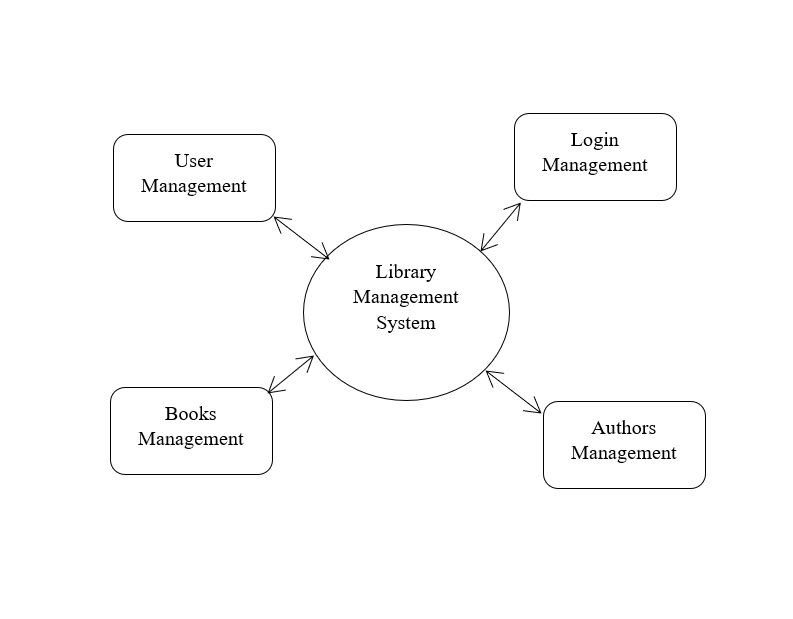
\includegraphics[scale=0.8]{./dfd-0} 
	\caption{First Level Data Flow Diagram}
	\label{fig:label} 
\end{figure}
\subsection{First Level DFD}
\begin{figure}[htb]
	\centering
	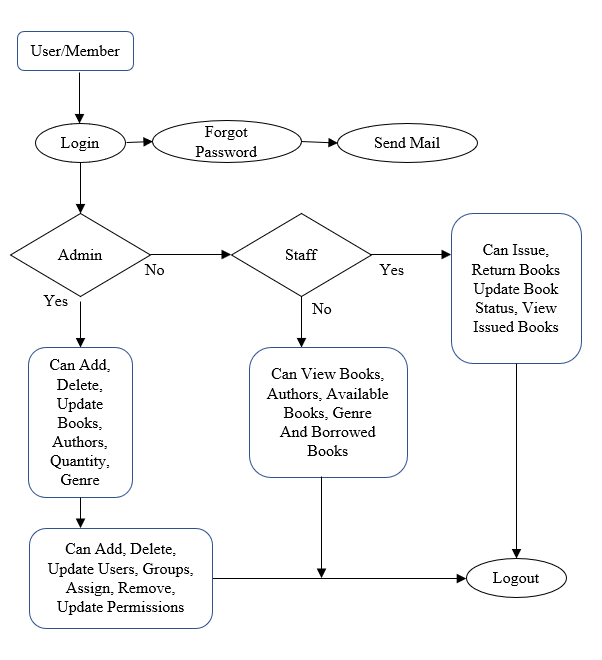
\includegraphics[scale=0.8]{./dfd-1} 
	\caption{Second Level Data Flow Diagram}
	\label{fig:label} 
\end{figure}

\newpage
\section{Entity Relationship Diagram}
\begin{figure}[htb]
	\centering
	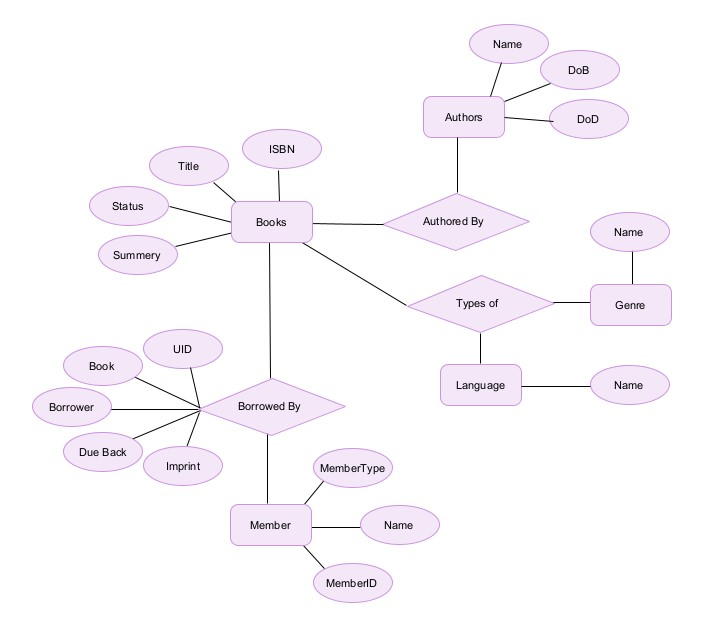
\includegraphics[scale=0.8]{./entity-relationship} 
	\caption{Entity Relationship Design}
	\label{fig:label} 
\end{figure}



\newpage
\section{Database Design}
\begin{figure}[htb]
	\centering
	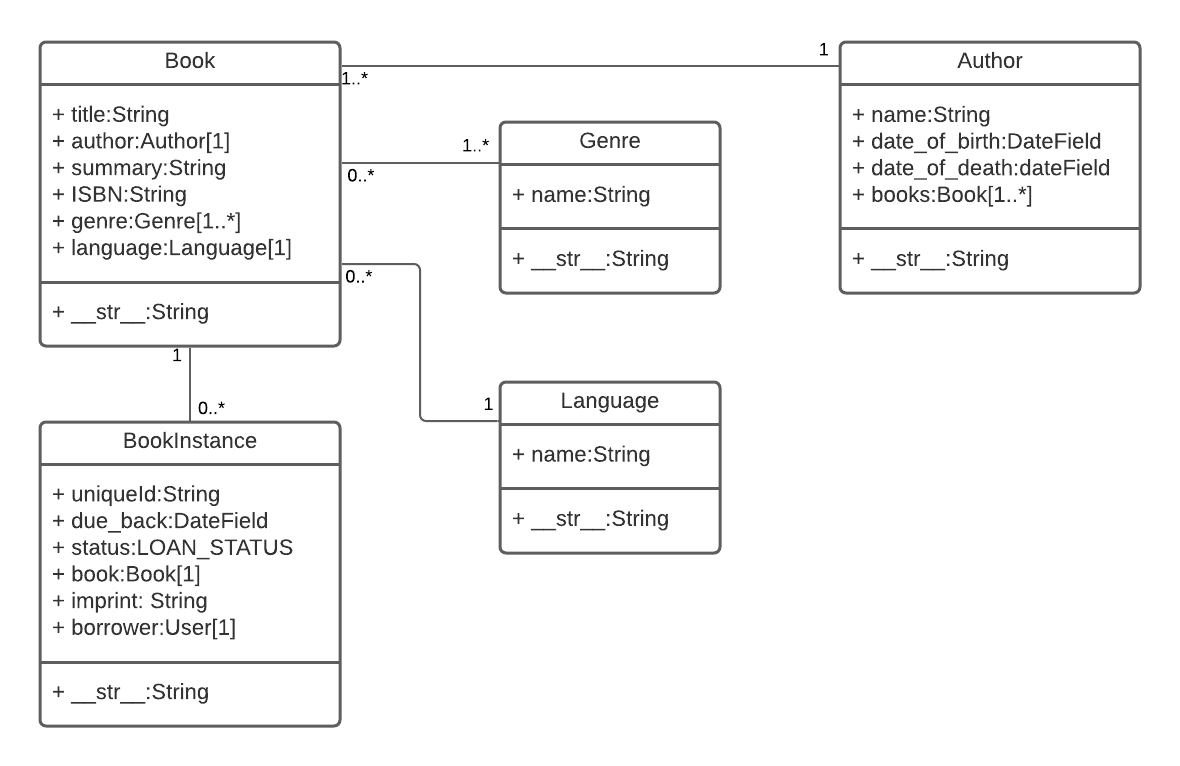
\includegraphics[scale=0.8]{./models} 
	\caption{Database Table Design}
	\label{fig:label} 
\end{figure}

\newpage
\chapter{Implementation}
\section{User Interface}
\begin{figure}[htb]
	\centering
	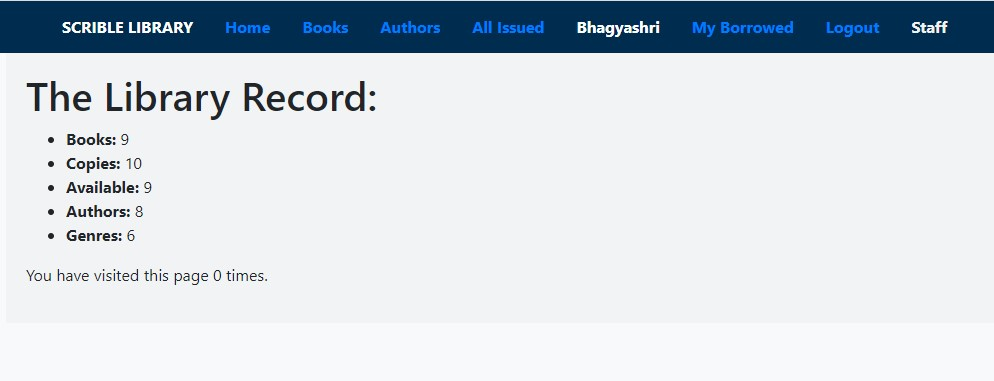
\includegraphics[scale=0.8]{./home} 
	\caption{The Library Record}
	\label{fig:label} 
\end{figure}

\newpage
\begin{figure}[htb]
	\centering
	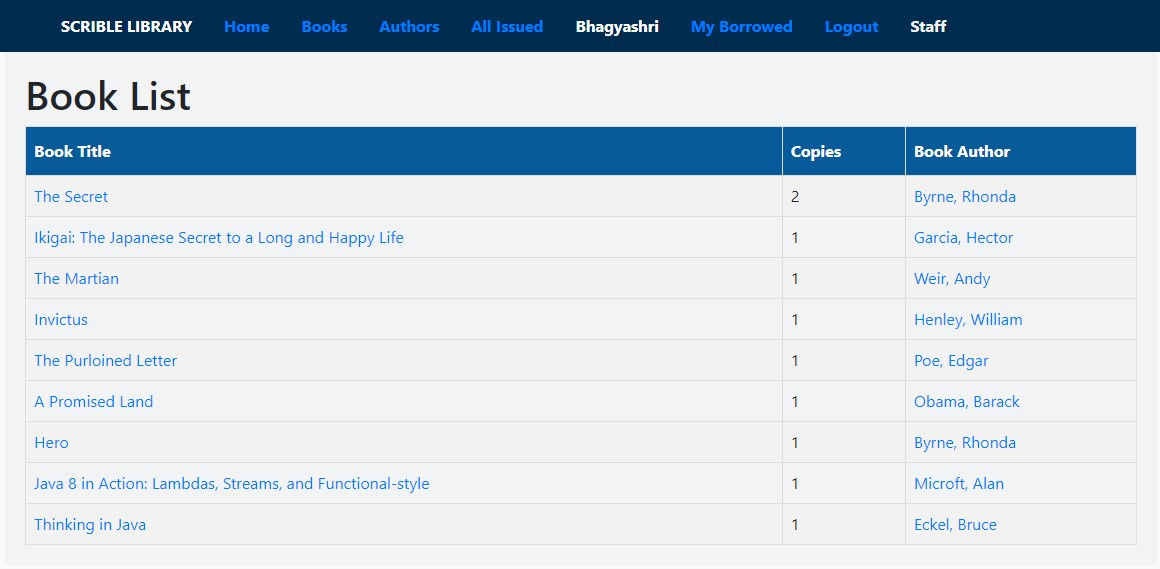
\includegraphics[width=12cm, height=6cm, angle=90]{./books} 
	\caption{Books List}
	\label{fig:label} 
\end{figure}
\newpage
\begin{figure}[htb]
	\centering
	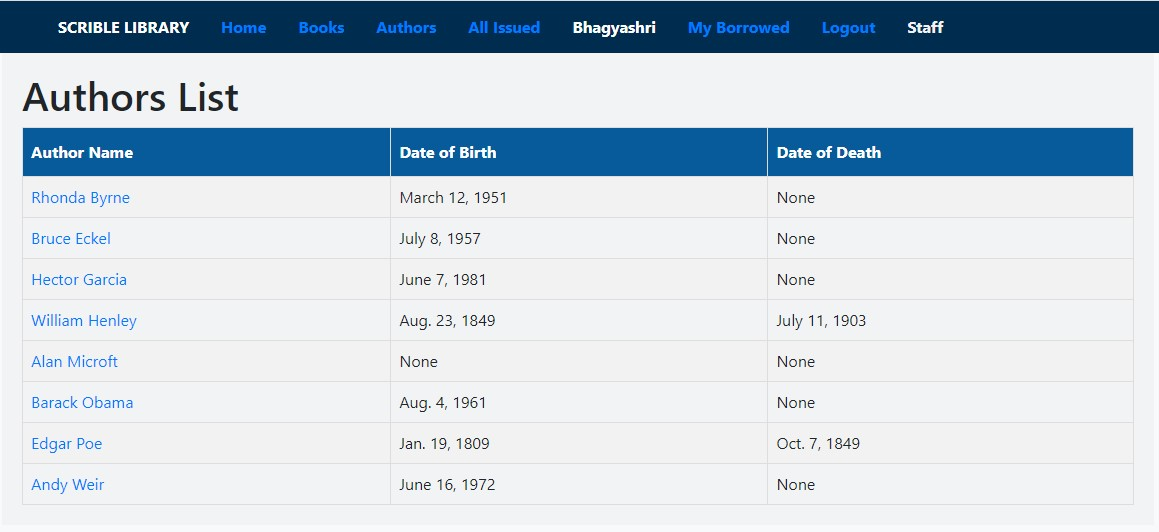
\includegraphics[scale=0.4, angle=90]{./authors} 
	\caption{Authors List}
	\label{fig:label} 
\end{figure}
\newpage
\begin{figure}[htb]
	\centering
	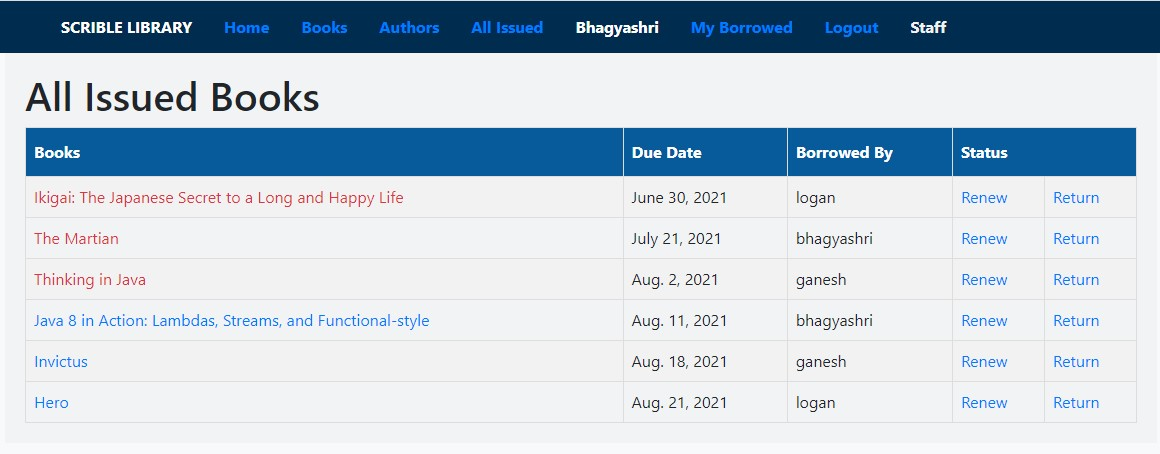
\includegraphics[scale=0.4, angle=90]{./issued} 
	\caption{All Issued Books}
	\label{fig:label} 
\end{figure}
\newpage
\begin{figure}[htb]
	\centering
	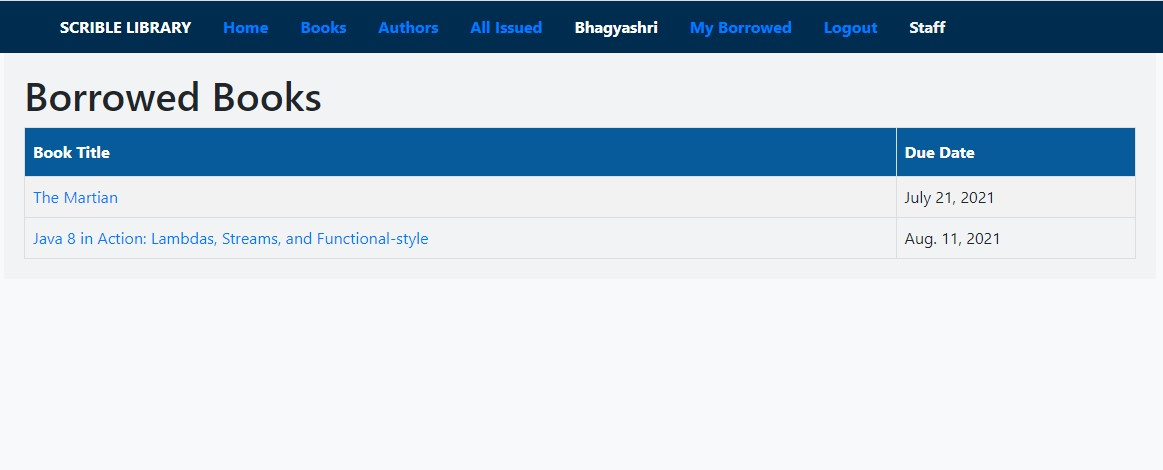
\includegraphics[scale=0.4, angle=90]{./borrowed} 
	\caption{Books Borrowed By Staff}
	\label{fig:label} 
\end{figure}
\newpage
\begin{figure}[htb]
	\centering
	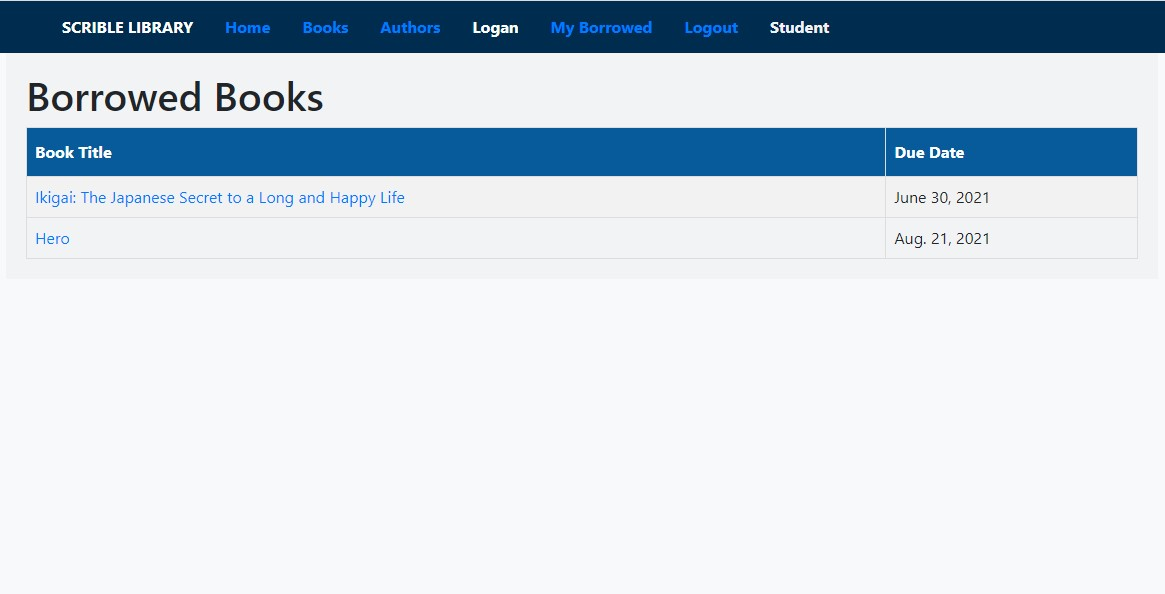
\includegraphics[scale=0.4, angle=90]{./students} 
	\caption{Books Borrowed By Students}
	\label{fig:label} 
\end{figure}

\newpage
\section{Technologies Used}

In this Section we will do Analysis of Technologies to use for implementing the project.
\subsection{Front End}
\subsubsection{HTML}
Hypertext Markup Language (HTML) is the standard markup language for documents designed to
be displayed in a web browser. It can be assisted by technologies such as Cascading Style Sheets
(CSS) and scripting languages such as JavaScript.
Web browsers receive HTML documents from a
web server or from local storage and render the documents into multimedia web pages. HTML
describes the structure of a web page semantically and originally included cues for the appearance
of the document.
HTML elements are the building blocks of HTML pages.\par With HTML constructs, images and other
objects such as interactive forms may be embedded into the rendered page. HTML provides a
means to create structured documents by denoting structural semantics for text such as headings,
paragraphs, lists, links, quotes and other items. HTML elements are delineated by tags, written
using angle brackets. Tags such as img and input directly introduce content into the page.
Other tags such as p surround and provide information about document text and may include
other tags as sub-elements. Browsers do not display the HTML tags, but use them to interpret the
content of the page.
HTML can embed programs written in a scripting language such as JavaScript, which affects the
behavior and content of web pages. Inclusion of CSS defines the look and layout of content. The
World Wide Web Consortium (W3C), former maintainer of the HTML and current maintainer of the
CSS standards, has encouraged the use of CSS over explicit presentational HTML since 1997.
 
\subsubsection{JavaScript}
JavaScript s a high-level, interpreted scripting language that conforms to the ECMAScript
specification. JavaScript has curly-bracket syntax, dynamic typing, prototype-based objectorientation,
and first-class functions.Alongside HTML and CSS, JavaScript is one of the core
technologies of the World Wide Web. JavaScript enables interactive web pages and is an essential
part of web applications.\par The vast majority of websites use it, and major web browsers have a
dedicated JavaScript engine to execute it. As a multi-paradigm language, JavaScript supports eventdriven,
functional, and imperative (including object-oriented and prototype-based) programming
styles. It has APIs for working with text, arrays, dates, regular expressions, and the DOM, but the
language itself does not include any I/O, such as networking, storage, or graphics facilities. It relies
upon the host environment in which it is embedded to provide these features.
\par Initially only implemented client-side in web browsers, JavaScript engines are now embedded in
many other types of host software, including server-side in web servers and databases, and in nonweb
programs such as word processors and PDF software, and in runtime environments that make
JavaScript available for writing mobile and desktop applications, including desktop widgets.
The terms Vanilla JavaScript and Vanilla JS refer to JavaScript not extended by any frameworks or
additional libraries. Scripts written in Vanilla JS are plain JavaScript code.Google's Chrome
extensions, Opera's extensions, Apple's Safari 5 extensions, Apple's Dashboard Widgets, Microsoft's
Gadgets, Yahoo! Widgets, Google Desktop Gadgets, and Serence Klipfolio are implemented using
JavaScript.

\subsubsection{CSS}
Cascading Style Sheets (CSS) is a style sheet language used for describing the presentation of a
document written in a markup language like HTML.CSS is a cornerstone technology of the World
Wide Web, alongside HTML and JavaScript.CSS is designed to enable the separation of
presentation and content, including layout, colors, and fonts.This separation can improve content
accessibility, provide more flexibility and control in the specification of presentation characteristics,
enable multiple web pages to share formatting by specifying the relevant CSS in a separate .css file,
and reduce complexity and repetition in the structural content.
\par One of the goals of CSS is to allow users greater control over presentation. Someone who finds red
italic headings difficult to read may apply a different style sheet. Depending on the browser and the
web site, a user may choose from various style sheets provided by the designers, or may remove all
added styles and view the site using the browser's default styling, or may override just the red italic
heading style without altering other attributes.


\subsection{Backend}
\subsubsection{Python}
Python is an interpreted, high-level, general-purpose programming language. Created by \textbf{Guido van
Rossum} and first released in 1991, Python's design philosophy emphasizes code readability with its
notable use of significant whitespace. Its language constructs and object-oriented approach aim to
help programmers write clear, logical code for small and large-scale projects.Python is dynamically
typed and garbage-collected. It supports multiple programming paradigms, including procedural,
object-oriented, and functional programming. Python is often described as a "batteries included"
language due to its comprehensive standard library.
\par Python was conceived in the late 1980s as a successor to the ABC language. Python 2.0, released
2000, introduced features like list comprehensions and a garbage collection system capable of
collecting reference cycles. Python 3.0, released 2008, was a major revision of the language that is
not completely backward-compatible, and much Python 2 code does not run unmodified on Python
3. Due to concern about the amount of code written for Python 2, support for Python 2.7 (the last
release in the 2.x series) was extended to 2020. Language developer Guido van Rossum shouldered
sole responsibility for the project until July 2018 but now shares his leadership as a member of a
five-person steering council.
\par Python interpreters are available for many operating systems. A global community of programmers
develops and maintains CPython, an open source[32] reference implementation. A non-profit
organization, the Python Software Foundation, manages and directs resources for Python and
CPython development.

\subsubsection{Django}
Django is a high-level Python web framework that enables rapid development of secure and maintainable websites. Built by experienced developers, Django takes care of much of the hassle of web development, so you can focus on writing your app without needing to reinvent the wheel. It is free and open source, has a thriving and active community, great documentation, and many options for free and paid-for support. \newline Django helps you write software that is:
\begin{itemize}
\item Complete - Django follows the "Batteries included" philosophy and provides almost everything developers might want to do "out of the box". Because everything you need is part of the one "product", it all works seamlessly together, follows consistent design principles, and has extensive and up-to-date documentation.
\item Versatile - Django can be (and has been) used to build almost any type of website — from content management systems and wikis, through to social networks and news sites. It can work with any client-side framework, and can deliver content in almost any format (including HTML, RSS feeds, JSON, XML, etc). The site you are currently reading is built with Django!
\item Secure - Django helps developers avoid many common security mistakes by providing a framework that has been engineered to "do the right things" to protect the website automatically. For example, Django provides a secure way to manage user accounts and passwords, avoiding common mistakes like putting session information in cookies where it is vulnerable (instead cookies just contain a key, and the actual data is stored in the database) or directly storing passwords rather than a password hash.

\item Scalable - Django uses a component-based “shared-nothing” architecture (each part of the architecture is independent of the others, and can hence be replaced or changed if needed). Having a clear separation between the different parts means that it can scale for increased traffic by adding hardware at any level: caching servers, database servers, or application servers. Some of the busiest sites have successfully scaled Django to meet their demands (e.g. Instagram and Disqus, to name just two).
\item Maintainable - Django code is written using design principles and patterns that encourage the creation of maintainable and reusable code. In particular, it makes use of the Don't Repeat Yourself (DRY) principle so there is no unnecessary duplication, reducing the amount of code. Django also promotes the grouping of related functionality into reusable "applications" and, at a lower level, groups related code into modules (along the lines of the Model View Controller (MVC) pattern).
\item Portable - Django is written in Python, which runs on many platforms. That means that you are not tied to any particular server platform, and can run your applications on many flavours of Linux, Windows, and Mac OS X. Furthermore, Django is well-supported by many web hosting providers, who often provide specific infrastructure and documentation for hosting Django sites.
\end{itemize}

\subsubsection{SQLite}
SQLite is a relational database management system (RDBMS) contained in a C library. In contrast to many other database management systems, SQLite is not a client–server database engine. Rather, it is embedded into the end program.

\par SQLite generally follows PostgreSQL syntax. SQLite uses a dynamically and weakly typed SQL syntax that does not guarantee the domain integrity. This means that one can, for example, insert a string into a column defined as an integer. SQLite will attempt to convert data between formats where appropriate, the string "123" into an integer in this case, but does not guarantee such conversions and will store the data as-is if such a conversion is not possible.

\par SQLite is a popular choice as embedded database software for local/client storage in application software such as web browsers. It is arguably the most widely deployed database engine, as it is used today by several widespread browsers, operating systems, and embedded systems (such as mobile phones), among others. SQLite has bindings to many programming languages.


\par SQLite is used almost everywhere from features phones to satellites etc. There are many applications of SQLite such as in Middleware, WebBrowsers, Web Application Framework, Mobile Operating Systems such as Blackberry OS, Android OS, Symbian OS, Linux, Windows etc. Also various Applications such as Adobe Photoshop Lightroom, Apple Photos, Evernote, Skype etc. Programming Languages such as python, AppleScript, Kotlin, Java etc.

\chapter{Performance Evaluation}
\section{System Testing}
System testing of software or hardware is testing conducted on a complete, integrated system to
evaluate the system's compliance with its specified requirements. System testing falls within the
scope of black-box testing, and as such, should require no knowledge of the inner design of the code
or logic. \par As a rule, system testing takes, as its input, all of the "integrated" software components that have passed integration testing and also the software system itself integrated with any applicable
hardware system(s). The purpose of integration testing is to detect any inconsistencies between the
software units that are integrated together (called assemblages) or between any of
the assemblages and the hardware. \par System testing is a more limited type of testing; it seeks to detect
defects both within the "inter-assemblages" and also within the system as a whole.
System testing is performed on the entire system in the context of a Functional
Requirement Specification(s) (FRS) and/or a System Requirement Specification (SRS). System
testing tests not only the design, but also the behavior and even the believed expectations of the
customer. It is also intended to test up to and beyond the bounds defined in the software/hardware
requirements specification(s).

\section{Black Box Testing}

Black Box Testing is a software testing method in which the functionalities of software applications are tested without having knowledge of internal code structure, implementation details and internal paths. Black Box Testing mainly focuses on input and output of software applications and it is entirely based on software requirements and specifications. It is also known as Behavioral Testing.

The above Black-Box can be any software system you want to test. For Example, an operating system like Windows, a website like Google, a database like Oracle or even your own custom application. Under Black Box Testing, you can test these applications by just focusing on the inputs and outputs without knowing their internal code implementation. 
Here are the generic steps followed to carry out any type of Black Box Testing.
\begin{itemize}
	\item Initially, the requirements and specifications of the system are examined.
	\item Tester chooses valid inputs (positive test scenario) to check whether SUT processes them correctly. Also, some invalid inputs (negative test scenario) are chosen to verify that the SUT is able to detect them.
	\item Tester determines expected outputs for all those inputs.
	\item Software tester constructs test cases with the selected inputs.
	\item The test cases are executed.
	\item Software tester compares the actual outputs with the expected outputs.
	\item Defects if any are fixed and re-tested.
	 
\end{itemize}

\subsection{Types of Black Box Testing}
There are many types of Black Box Testing but the following are the prominent ones -
\begin{itemize}
	\item \textbf{Functional testing} - This black box testing type is related to the functional requirements of a system; it is done by software testers.
	\item \textbf{Non-functional testing} - This type of black box testing is not related to testing of specific functionality, but non-functional requirements such as performance, scalability, usability.
	\item \textbf{Regression testing} - Regression Testing is done after code fixes, upgrades or any other system maintenance to check the new code has not affected the existing code.
	
\end{itemize}


\section{Testing Strategy}

A Test Strategy is a plan for defining an approach to the Software Testing Life Cycle (STLC). It guides teams to define Test Coverage and testing scope. It helps testers get a clear picture of the project at any instance. The possibility of missing any test activity is very low when there is a proper test strategy in place.

\subsection{Test Strategy Document}
Test Strategy Document is a well-described document in software testing which clearly defines the exact software testing approach and testing objectives of the software application. Test document is an important document for QA teams which is derived from actual business requirements that guides the whole team about software testing approach and objectives for each activity in the software testing process.

A Test strategy document answers all the questions like what you want to get done and how you are going to accomplish it, etc. Writing an effective Strategy document is a skill that a tester develops with experience. Testing strategy plan should be communicated with the entire team so that the team will be consistent on approach and responsibilities.\newline
Following are the prominent Test Strategy used in Black box Testing
\begin{enumerate}
	\item \textbf{Equivalence Class Testing:} It is used to minimize the number of possible test cases to an optimum level while maintains reasonable test coverage.
	\item \textbf{Boundary Value Testing:} Boundary value testing is focused on the values at boundaries. This technique determines whether a certain range of values are acceptable by the system or not. It is very useful in reducing the number of test cases. It is most suitable for the systems where an input is within certain ranges.
	\item \textbf{Decision Table Testing}: A decision table puts causes and their effects in a matrix. There is a unique combination in each column.
	
\end{enumerate}

